\section{The Two Norms}

\begin{frame}{Two Norms of Interest}

    There are two most widely used norms that we are interested in:
    ~\\~\\
    \begin{itemize}
        \item The $\ell_1$-norm
        \item The $\ell_2$-norm
    \end{itemize}
    
\end{frame}

\begin{frame}{The \texorpdfstring{$\ell_1$}~-Norm}

    
    Replacing $n$ of equation \ref{eqn:general} with 1, i.e. using the absolute values will result in $\ell_1$-norm. So, the following would be $\ell_1$ regularized cost functions: 
    ~\\~\\
    \begin{equation}
    \label{eqn:l1}
        \minimize{x} \quad \left\|Ax-b\right\|_2^2+\lambda \left\|x\right\|_1
    \end{equation}
    
\end{frame}

\begin{frame}{The \texorpdfstring$\ell_2$-Norm}

    Replacing $n$ of equation \ref{eqn:general} with $2$, i.e. using the squared values of the weights, will result in $\ell_2$-norm. So, the following would be $\ell_2$ regularized cost functions: 
    ~\\~\\
    \begin{equation}
    \label{eqn:l2}
        \minimize{x} \quad \left\|Ax-b\right\|_2^2+\lambda \left\|x\right\|_2
    \end{equation}
\end{frame}

\subsection{Comparison Between the Two Norms}

\begin{frame}{Comparison}

    \vspace*{\fill}
    \begin{center}

        \begin{table}[!ht]
        \centering
            \begin{tabular}{|c|c|c|}
            \hline
                ~&\texorpdfstring{$\ell_1$} ~-Norm&\texorpdfstring{$\ell_2$} ~-Norm \\
                \hline
                Sparsity (See Fig \ref{sparsity}) & Yes & No\\
                \hline
                Robustness & Yes & No\\
                \hline
            \end{tabular}
        \caption{Differences between the two norms}
        \end{table}
    \vfill
    \end{center}
    
\end{frame}

\begin{frame}{Sparsity of \texorpdfstring{$\ell_1$} ~-Norm}

    ~\\
    \begin{figure}[h!] 
        
        \centering
        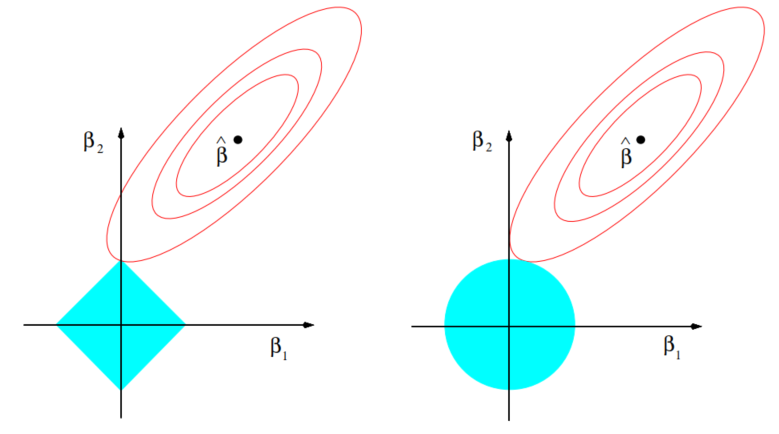
\includegraphics[width=0.5\linewidth]{images/sparsity.png}
        \caption{Contours of error and constraint functions for Lasso (Left) and Ridge Regression (Right) \cite{Hastie2001elements}. }
        \vspace{4ex}
        \label{sparsity}
    \end{figure}
\end{frame}